\chapter{Strategy Extraction}
\label{ch:strategy}

\newcommand{\strategyext}[0]{\textsc{StrategyGen}\xspace}
\newcommand{\genstrategy}{\textsc{StrategyGen}}
\newcommand{\strategy}[0]{\textsc{Strategy}\xspace}
\newcommand{\partition}[0]{\textsc{Partition}\xspace}
\newcommand{\nextf}[0]{\textsc{Next}\xspace}
\newcommand{\ogametree}[0]{\mbox{\sc OppGT}}
\newcommand{\eagametree}[0]{\mbox{\sc AbsGT}'}
\newcommand{\pgametree}[0]{\mbox{\sc Cand}}
\newcommand{\apgametree}[0]{\mbox{\sc AbsSolvedGT}}
\newcommand{\opgametree}[0]{\mbox{\sc Spoiling}}

\renewcommand{\ss}[0]{\mathbf{s}}
\newcommand{\cc}[0]{\mathbf{c}}
\newcommand{\uu}[0]{\mathbf{u}}

\newtheorem{theorem}{Theorem}
\newtheorem{example}{Example}
\newtheorem{proposition}{Proposition}

In the previous chapter I introduced an algorithm for solving realisability for bounded safety games. In most applications of synthesis it is desirable to construct a controller strategy rather than merely prove its existence. In this chapter I will introduce a strategy extraction procedure that complements the bounded reachability algorithm. This process takes abstract game trees generated during reachability analysis and, using Craig interpolation, extracts mappings of states to player actions. By using interpolation this step can be done efficiently.

The problem solved in this chapter is related to the extraction of a Skolem function for a QBF. Recall from Chapter~\ref{ch:background} that a Skolem function $f$ provides a mapping from a prefix of universal variables $\hat{y}_0, \hat{y_1}, ..., \hat{y_i}$ to existential variables $\hat{x}$ such that when substituting $\hat{x}$ for $f(\hat{y}_0, \hat{y_1}, ..., \hat{y_i})$ the QBF is equisatisfiable. A Skolem function for a bounded realisability QBF gives a mapping from a prefix of past environment actions to a controller action, i.e. a strategy for that game round. A strategy for the entire game consists of a Skolem function for every round. In this chapter, we construct a strategy by replacing the prefix of previous environment actions with a game state and current environment action pair. This allows us to solve a simpler problem than Skolemisation of the entire QBF by once again taking advantage of the structure of the bounded realisability QBF.

\section{Algorithm}

In this chapter we will assume that the safety game is winning for the controller. However, the technique is also easily applied to the environment to extract a spoiling strategy. In computing realisability of a safety game the algorithm constructs a \emph{certificate tree}, which is an abstract game tree $T$ such that for a set of states $s$ and game bound $\kappa$, $s \land \textsc{\textoverline{treeFormula}}(\kappa, \textsc{extend}(T))$ is false. In other words it is a game abstraction for which the environment has no candidate strategy.

We use the certificate tree computed by the game solver as a starting point for strategy generation.  We know that the controller can win the game in $\kappa$ rounds by picking actions from the tree; however we do not yet know exactly which actions should be picked in every state.


\subsection{Example}

Figure~\ref{fig:stratExample} introduces the running example for this chapter. It shows a state machine for a game $(S, \mathcal{U}, \mathcal{C}, \delta, s_0)$ where $S$ consists of two one bit variables \texttt{p} and \texttt{e}, $\mathcal{U}$ and $\mathcal{C}$ each consist of a single one bit variable \texttt{u} and \texttt{c} respectively. The diagram shows $\delta$ as a deterministic finite state automaton with edges labelled by a tuple (\texttt{u}, \texttt{c}). We use \texttt{*} as a wildcard value to simplify the presentation. The game is simple, \texttt{p} is set to the previous value of \texttt{u} and \texttt{e} is set to \texttt{1} when $\texttt{c} \neq \texttt{p}$. The initial state, $s_0$, is $\texttt{p} = 0 \land \texttt{e} = 0$ and the error set is $\texttt{e} = 1$. In other words, the controller must simply match the previous action of the environment to avoid the error set.

\tikzset{
    pil/.style={
        -{Latex[length=3mm]},
        thick
    },
    snode/.style={
        align=center,
        circle,
        draw,
        thick
    }
}

\begin{figure}
    \centering
    \begin{tikzpicture}
        \node [snode]
            (s0){\texttt{p=0} \\ \texttt{e=0}};
        \node [draw=none,left=of s0] (i){};
        \node [snode,right=1.5cm of s0]
            (s1){\texttt{p=1} \\ \texttt{e=0}};
        \node [snode,accepting,below=1cm of s0]
            (err){\texttt{p=*} \\ \texttt{e=1}};

        \draw [pil] (i) edge (s0);
        \draw [pil] (s0) edge [bend left] node [above] {$(1, 0)$} (s1);
        \draw [pil] (s0) edge node [left] {$(*, 1)$} (err);
        \draw [pil] (s0) edge [loop above] node [above] {$(0, 0)$} (s0);
        \draw [pil] (s1) edge node [below right] {$(*, 0)$} (err);
        \draw [pil] (s1) edge [loop above] node [above] {$(1, 1)$} (s1);
        \draw [pil] (s1) edge [bend left] node [above] {$(0, 1)$} (s0);
        \draw [pil] (err) edge [loop left] node [below right=10pt and -3pt] {$(*, *)$} (err);
    \end{tikzpicture}
    \caption{Transition relation of the running example}
    \label{fig:stratExample}
\end{figure}

The strategy generation algorithm takes an initial set $s$ and its certificate tree $T$, computed by the game solver, and generates a winning controller strategy starting from $s$.  To this end, it first partitions $s$ into subsets $s_i$, one for each outgoing branch of $T$ (Figure~\ref{fig:partition}), such that the controller can win from $s_i$ by picking action $c_i$ along the $i$th branch of the tree.  This partitioning defines the local winning strategy in the root node of $T$.  Next, for each partition $s_i$, the algorithm computes the set of $c_i$-successor states of $s_i$, obtaining the set $s_i'$ of states winning in the child subtree $T_i'$ of $T_i$ (Figure~\ref{fig:partition}).  The algorithm is then invoked recursively for each subtree $T_i'$.

\begin{figure}[b]
    \centering
    \captionsetup[subfigure]{width=\textwidth,justification=raggedleft}
    \hspace*{\fill}%
    \begin{subfigure}[t]{.4\textwidth}
        \centering
        \begin{minipage}[t][3cm][t]{\textwidth}
        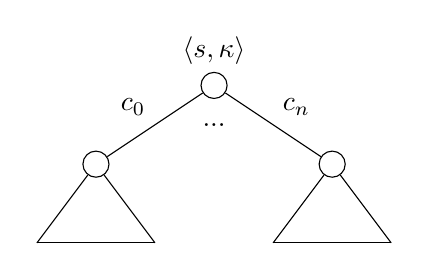
\begin{tikzpicture}[level distance = 10mm,baseline]
            \node [circle,draw] (root){}
                child {node [circle,draw] (left0){}
                    child {node (left1){}
                        edge from parent [draw=none]
                    }
                    child {node (left2){}
                        edge from parent [draw=none]
                    }
                    edge from parent node [above left] {$c_0$}
                }
                child {node [circle] {}
                    edge from parent [draw=none] node [] {$...$}
                }
                child {node [circle,draw] (right0){}
                    child {node (right1){}
                        edge from parent [draw=none]
                    }
                    child {node (right2){}
                        edge from parent [draw=none]
                    }
                    edge from parent node [above right] {$c_n$}
                }
                node [left=4pt] {}
                node [above=4pt] {$\langle s, \kappa \rangle$};

            \draw (left1.center) -- (left2.center);
            \draw (left0) -- (left1.center);
            \draw (left0) -- (left2.center);
            \draw (right1.center) -- (right2.center);
            \draw (right0) -- (right1.center);
            \draw (right0) -- (right2.center);
        \end{tikzpicture}
        \end{minipage}
        \caption{Before}
    \end{subfigure}\hfill%
    \begin{subfigure}[t]{.3\textwidth}
        \centering
        \begin{minipage}[t][3cm][t]{\textwidth}
        \begin{tikzpicture}[level distance = 10mm,baseline]
            \node [circle,draw] (root){}
                child {node [circle,draw] (left0){}
                    child {node (left1){}
                        edge from parent [draw=none]
                    }
                    child {node (left2){}
                        edge from parent [draw=none]
                    }
                    edge from parent node [left] {$c_0$}
                }
                node [above=4pt] {$\langle s_0, \kappa \rangle$};

            \node [draw=none,below right=25pt and 22pt] {$...$};

            \begin{scope}[xshift=60pt]
            \node [circle,draw] (root2){}
                child {node [circle,draw] (right0){}
                    child {node (right1){}
                        edge from parent [draw=none]
                    }
                    child {node (right2){}
                        edge from parent [draw=none]
                    }
                    edge from parent node [right] {$c_n$}
                }
                node [left=4pt] {}
                node [above=4pt] {$\langle s_n, \kappa \rangle$};
            \end{scope}

            \node [below=5pt of left0] {$T_0$};
            \node [below=5pt of right0] {$T_n$};
            \draw (left1.center) -- (left2.center);
            \draw (left0) -- (left1.center);
            \draw (left0) -- (left2.center);
            \draw (right1.center) -- (right2.center);
            \draw (right0) -- (right1.center);
            \draw (right0) -- (right2.center);
        \end{tikzpicture}
        \end{minipage}
        \caption{After}
    \end{subfigure}%
    \hspace*{\fill}
    \caption{Partitioning}
    \label{fig:partition}
\end{figure}

Figure~\ref{fig:algex} illustrates operation of the algorithm on the winning abstract game tree returned by the game solver for our running example (Figure~\ref{fig:stratExample}).  The algorithm starts at the root of the tree and the initial set $I=\{s_0\}$.  The game tree only defines one winning action in the root node, hence this action is winning in all states of $I$ and no partitioning is required.  We compute the successor set reachable by playing action $0$ in $I$: $I' = \textsc{succ}(I, i) = \{s_1, s_2\}$.

%%%(see the game automaton in Figure~\ref{f:exm:delta}(a)).

\tikzset{every node/.style={solid}}
\tikzstyle{fixed}=[solid]
\begin{figure}[b]
    \centering
    \captionsetup[subfigure]{width=\textwidth,justification=raggedleft}
    \begin{subfigure}[t]{.4\textwidth}
        \centering
        \begin{minipage}[t][4cm][t]{\textwidth}
        \begin{tikzpicture}[dash pattern = on 2pt off 2pt, level distance = 10mm,baseline]
            \node [circle,draw] (root){}
                child {node [circle,draw] {}
                    child {node [circle,draw] {}
                        child {node [circle,draw,right=5pt] {}
                            edge from parent [fixed] node [left] {\texttt{0}}
                        }
                        child {node [circle,draw,left=5pt] {}
                            edge from parent [fixed] node [right] {\texttt{1}}
                        }
                        edge from parent [fixed] node [left] {\texttt{0}}
                    }
                    child {node [circle,draw] {}
                        child {node [circle,draw,right=5pt] {}
                            edge from parent [fixed] node [left] {\texttt{0}}
                        }
                        child {node [circle,draw,left=5pt] {}
                            edge from parent [fixed] node [right] {\texttt{1}}
                        }
                        edge from parent [fixed] node [right] {\texttt{1}}
                    }
                    edge from parent [fixed] node [left] {\texttt{0}}
                }
                node [left=4pt] {}
                node [above=4pt] {$\langle s, 3 \rangle$};
        \end{tikzpicture}
        \end{minipage}
        \caption{AGT}
        \label{fig:algexa}
    \end{subfigure}
    \begin{subfigure}[t]{.4\textwidth}
        \centering
        \begin{minipage}[t][4cm][t]{\textwidth}
        \begin{tikzpicture}[dash pattern = on 2pt off 2pt, level distance = 10mm,baseline]
            \node [circle,draw] (root){}
                child {node [circle,draw] {}
                    child {node [circle,draw] {}
                        edge from parent [fixed] node [left] {\texttt{i}}
                    }
                    edge from parent [fixed] node [left] {\texttt{a}}
                }
                child {node [circle,draw] {}
                    child {node [circle,draw] {}
                        edge from parent [fixed] node [right] {\texttt{c}}
                    }
                    edge from parent [fixed] node [right] {\texttt{b}}
                }
                node [left=4pt] {}
                node [above=4pt] {$\langle s, 2 \rangle$};
        \end{tikzpicture}
        \end{minipage}
        \caption{AGT}
        \label{fig:algexb}
    \end{subfigure}

    \begin{subfigure}[t]{.4\textwidth}
        \centering
        \begin{minipage}[t][4cm][t]{\textwidth}
        \begin{tikzpicture}[dash pattern = on 2pt off 2pt, level distance = 10mm,baseline]
            \node [circle,draw] (root){}
                child {node [circle,draw] {}
                    child {node [circle,draw] {}
                        edge from parent [fixed] node [left] {\texttt{i}}
                    }
                    edge from parent [fixed] node [left] {\texttt{a}}
                }
                node [above=4pt] {$\langle s, 2 \rangle$};

            \node [circle,draw,right=2cm] (root){}
                child {node [circle,draw] {}
                    child {node [circle,draw] {}
                        edge from parent [fixed] node [right] {\texttt{c}}
                    }
                    edge from parent [fixed] node [right] {\texttt{b}}
                }
                node [right=2.2cm,above=4pt] {$\langle s, 2 \rangle$};
        \end{tikzpicture}
        \end{minipage}
        \caption{AGT}
        \label{fig:algexc}
    \end{subfigure}
    \begin{subfigure}[t]{.4\textwidth}
        \centering
        \begin{minipage}[t][3cm][t]{\textwidth}
        \begin{tikzpicture}[level distance = 10mm,baseline]
            \node [circle] (root){}
                child {node [circle,draw] {}
                    child {node [circle,draw] {}
                        edge from parent [fixed] node [left] {\texttt{i}}
                    }
                    node [above=4pt] {$\langle s, 2 \rangle$}
                    edge from parent [draw=none]
                };

            \node [circle,right=2cm] (root){}
                child {node [circle,draw] {}
                    child {node [circle,draw] {}
                        edge from parent [fixed] node [right] {\texttt{c}}
                    }
                    node [above=4pt] {$\langle s, 2 \rangle$}
                    edge from parent [draw=none]
                };
        \end{tikzpicture}
        \end{minipage}
        \caption{AGT}
        \label{fig:algexd}
    \end{subfigure}

    \caption{Operation of the strategy extraction algorithm on the example}
    \label{fig:algex}
\end{figure}


%%%\begin{figure}[t]
%%%    \centering
%%%    \includegraphics[width=.8\linewidth]{example_abs_new_clones_cropped.pdf}
%%%    \vspace{-3mm}
%%%    \caption{Operation of the strategy extraction algorithm on the 
%%%    running example.}\label{f:algex}
%%%\end{figure}

Next, we descend down the $i$ branch of the tree and consider subtree $T'$ and its initial set $I'$ (Figure~\ref{fig:algexb}).  We partition $I'$ into subsets $I'_1=\{s_1\}$ and $I'_2=\{s_2\}$ that are winning for the left and right subtrees of $T'$ respectively, i.e., the controller must play action $0$ in state $s_1$ and $1$ in $s_2$.  Consider the resulting subtrees $T'_1$ and $T'_2$ with initial sets $I'_1$ and $I'_2$ (Figure~\ref{fig:algexc}).  We have $I''_1 = \textsc{succ}(I'_1, a) = \{s_4\}$, $I''_2 = \textsc{succ}(I'_2, b) = \{s_3\}$.  Finally, we obtain two subtrees $T''_1$ and $T''_2$ with initial sets $I''_1$ and $I''_2$ (Figure~\ref{fig:algexd}).  Both subtrees have one branch; hence corresponding actions $i$ and $c$ are winning in $I''_1$ and $I''_2$ respectively.

Putting together fragments of the winning strategy computed above, we obtain the following strategy for this example: $\pi(s_0)=i$, $\pi(s_1)=a$, $\pi(s_2)=b$, $\pi(s_3)=c$, $\pi(s_4)=i$.

The above algorithm involves two potentially costly operations: winning set partitioning and successor set computation.  If implemented na\"ively, these operations can lead to unacceptable performance.  The key insight behind our solution is that both operations can be efficiently approximated from the proof of unsatisfiability of the formula $E_T(I)$, with the help of interpolation, as described below.  The resulting approximations are sound, i.e., preserve the correctness of the resulting strategy.

\subsection{Local Strategies}

Algorithm~\ref{alg:strat} shows the pseudocode of the strategy generation algorithm.  The algorithm proceeds in two phases: the first phase (\textsc{GenLocalStrats}) computes local strategies in nodes of $T$; the second phase (\textsc{CompileStrat}) compiles all local strategies into a winning strategy function.

The \textsc{GenLocalStrats} function recursively traverses the certificate tree $T$, starting from the root, computing local strategies in each node.  The main operation of the algorithm, called \textsc{Partition}, splits $(T,I)$ into $j$ pairs $(T_i, I_i)$, as shown in Figure~\ref{f:partition}.  Each tree $T_i$ is a copy of a single branch of $T$.  The partitioning is constructed in such a way that the action $c_i$ that labels the root edge of $T_i$ is a winning controller action in $I_i$.

%%%\begin{figure}[t]
%%%    \centering
%%%    \includegraphics[width=.68\linewidth]{example_strategy_vars_cropped.pdf}
%%%    \vspace{-2mm}
%%%    \caption{The \textsc{Partition} function.\label{f:partition}}
%%%    \vspace{-3mm}
%%%\end{figure}

Next we consider each pair $(T_i, I_i)$
(lines~\ref{alg:strat:for}-\ref{alg:strat:endfor}). We descend
down the tree and compute the controller strategy in the child
subtree $T_i'$ of $T_i$ (right-hand side of Figure~\ref{f:partition}).
%By construction, the root of $T_i$ has exactly one outgoing edge
%labeled with the move $c_i$.
To do so, we first compute the set of $c_i$-successors of $I_i$:
More precisely, we compute an overapproximation $I_i'\supseteq
succ(I_i, c_i)$, such that $T_i'$ is a certificate
tree for $I_i'$.  Such an overapproximation is returned by the
\textsc{Next} function in line~\ref{alg:strat:next}.  We can now
recursively invoke the strategy generation function to compute a
winning strategy for the pair $(T_i', I_i')$
(line~\ref{alg:strat:rec}).

%\textsc{Next} computes $I_i'$ which is an invariant preserving
%overapproximation of states reachable from  $I_i$ if the
%controller plays $c_i$.  We will show that \textsc{Next} preserves
%the invariant: $T_i'$ is a certificate tree for $E(I_i')$.  We can
%now recursively invoke the strategy generation function to compute
%a winning strategy for the pair $(T_i', I_i')$

%The \textsc{GenLocalStrats} function recursively traverses the
%certificate tree, starting from the root, computing local
%strategies in each node.  The main operation of the algorithm,
%called \textsc{Partition}, takes a set $I$ and its certificate
%tree $T$ and produces $j$ pairs $(T_i, I_i)$, one for each branch
%of $T$, such that
%\begin{itemize}
%    \item Trees $T_i$ are obtained by splitting $T$ at the root node, as shown in Figure~\ref{}
%    \item Sets $I_i$ form a partitioning of $I$: $I=\bigvee I_i$ and $\forall i, k. (i\neq k) \implies I_i\land I_k=\bot$
%    \item $T_i$ is a certificate tree for $I_i$
%\end{itemize}
%
\begin{algorithm}[t]
   \caption{Computing a winning strategy}\label{alg:strat}
   \begin{algorithmic}[1]
%        \Statex \textbf{Input:}  Abstract game tree $T$ and a CNF $I$ over state
%        variables $s$.
%        \Statex \textbf{Precondition:} $T$ is a certificate of existence of a winning strategy
%        from the set $I$, i.e., $E_T(I)$ is unsatisfiable.
%        \Statex \textbf{Returns:} Winning controller strategy from set $I$.
        \Function{GenStrategy}{$T$, $I$}
            \State $Strat \gets \Call{GenLocalStrats}{T,I}$
            \State \Return{$\Call{CompileStrat}{Strat}$}
        \EndFunction
        \Statex

        \Function{GenLocalStrats}{$T$, $I$}
            \State $v \gets \Call{root}{T}$
            \State $[(e_1, a_1, v_1),\ldots,(e_j,a_j,v_j)] \gets \Call{edges}{v}$
            \State $[(T_1,I_1),\ldots,(T_j, I_j)] \gets \partition(T, I \land \neg O)$
            \State $Strat \gets \{(I_i, c_i, \Call{height}{T}) \mid i \in[1,j]\}$\label{alg:strat:strati}
            \For{$i = 1$ to $j$}\label{alg:strat:for}
                \State $(T_i', I_i') \gets \nextf(T_i, I_i)$\label{alg:strat:next}
                \State $Strat_i \gets \Call{GenLocalStrats}{T_i', I_i'}$\label{alg:strat:rec}
                \State $Strat \gets Strat \cup Strat_i$
            \EndFor\label{alg:strat:endfor}
            \State \Return{$Strat$} \label{alg:strat:return}
        \EndFunction
    \end{algorithmic}
\end{algorithm}
%
%Since each tree $T_i$ only allows a single controller action $c_i$
%in the root node and because $T_i$ is a certificate for $I_i$, we
%know that the controller can win the game by choosing action $c_i$
%in any state in $I_i$.  Thus, we obtain a winning strategy in $I$,
%which consists of playing action $c_i$ in each subset $I_i$.
%Line~\ref{alg:strat:strati} of Algorithm~\ref{} compiles this
%strategy into a symbolic form.  We represent the strategy as a
%pair of relations.  The first component of the pair is a partial
%function $F: S \rightarrow L_c$ that maps states to winning
%controller moves.  The second component is the set of states
%$W\subseteq S$ where $F$ is defined.
%
%Next we consider each pair $(T_i, I_i)$
%(lines~\ref{alg:strat:for}-\ref{alg:strat:endfor}). We descend
%down the tree and compute the controller strategy in the child
%subtree $T_i'$ of $T_i$ (Figure~\ref{}).  To do so, we first
%compute the set of $c_i$-successors of $I_i$:
%\begin{equation}\label{eq:succ}
%    succ(I_i, c_i) = \{\ss' \mid \exists \ss\in I_i,\uu\in L_u. \ss' = \delta(\ss, c_i, \uu)\}
%\end{equation}
%More precisely, we compute an overapproximation
%$I_i'\supseteq succ(I_i, c_i)$, such that $T_i'$ is a certificate
%tree for $I_i'$.  Such an overapproximation is returned by the
%\textsc{Next} function in line~\ref{alg:strat:next}.  We can now
%recursively invoke the strategy generation function to compute a
%winning strategy for the pair $(T_i', I_i')$
%(line~\ref{alg:strat:rec}).

The algorithm returns the set of tuples $(W, a, k)$.  Each tuple
represents a fragment of the strategy in some tree node, where $W$
is the winning set in this node, $a$ is the controller action to
play in this set, and $k$ is the distance from the node to the
bottom of the tree (i.e., distance to the goal).

%Finally, we combine all partial strategies produced by the
%algorithm into a winning controller strategy in
%line~\ref{alg:strat:return}.

%Algorithm~\ref{alg:strat} relies on two potentially costly operations:
%\textsc{Partition}, which generates a local strategy in a node,
%and \textsc{Next}, which computes an overapproximation of the
%successor set.  Below we describe how we implement both operations
%efficiently using interpolation.

\subsection{Partitioning game trees}

The \textsc{Partition} function
(Algorithm~\ref{alg:strat:partition}) computes a local strategy in
the root of an abstract game tree.  It takes a pair $(T,I)$, such
that $T$ is a certificate tree for set $I$ and partitions $I$ into
subsets $I_i$ such that the controller can win by choosing action
$c_i$ in $I_i$.

\begin{algorithm}[t]
   \caption{Partitioning winning states}\label{alg:strat:partition}
   \begin{algorithmic}[1]
        \Function{$\partition$}{$T$, $I$}
        \State $v \gets root(T)$
            \State $\hat{I} \gets I$, $\hat{T} \gets T$ \For{$i =
            1$ to $j$}
            \State $(T_i, \tilde{T}) \gets split(\hat{T})$\label{alg:partition:split}
            \State $A \gets E_{\tilde{T}}(\hat{I}) $ \label{alg:strat:partition:Bi}
            \State $B \gets E_{T_i}(\top)$\label{alg:strat:partition:Ai}
            \State $\mathcal{I}(s_v) \gets Interpolant(A, B)$\label{alg:partition:I}
            \State $I_i \gets \mathcal{I}(s) \land \hat{I}$\label{alg:partition:Ii}
            \State $\hat{I} \gets \hat{I} \land \neg\mathcal{I}(s)$,~~$\hat{T} \gets \tilde{T}$\label{alg:partition:upd}
            \EndFor
            \State \Return{$[(T_1, I_1),\ldots, (T_j, I_j)]$} \label{alg:strat:partition:return}
        \EndFunction
    \end{algorithmic}
\end{algorithm}

At every iteration, the algorithm splits the tree into the
leftmost branch $T_i$ and the remaining tree (Figure~\ref{f:split}).
It then computes the set $I_i$ where the controller wins by following
the branch $T_i$ and removes $I_i$ from the initial set $I$.  At the
next iteration it considers the leftover tree $\tilde{T_i}$ and the
shrunk initial set $\hat{I}$.

%%%\begin{figure}[t]
%%%    \centering
%%%    \includegraphics[width=.5\linewidth]{split_cropped.pdf}
%%%    \vspace{-2mm}
%%%    \caption{Splitting of $T$ in the \textsc{Partition} function.\label{f:split}}
%%%    \vspace{-3mm}
%%%\end{figure}


The algorithm maintains the invariant that $\hat{T}$ is a
certificate tree for $\hat{I}$ and hence $E_{\hat{T}}(\hat{I})$ is
unsatisfiable.  We decompose this formula into two conjuncts
$E_{\hat{T}}(\hat{I}) =A \land B$ such that $A$ and $B$ only share
state variables $s_v$ in the root node $v$ of $T$ and that the
interpolant $\mathcal{I}$ of $A$ and $B$ consists of states where
the controller can win by following the $T_i$ subtree.  Hence
$\mathcal{I}\land \hat{I}$ gives us the desired set $I_i$.

Informally, $A$ is a partial expansion of the game formula induced by
$\tilde{T}$.  It is satisfiable iff there exists a spoiling environment
strategy from $\hat{I}$ against abstract game tree $\tilde{T}$.
$B$ is a partial expansion of the game induced by $T_i$.  It is satisfiable
iff there exists a spoiling environment strategy against $T_i$.
Both $A$ and $B$ can be satisfiable individually, but their conjunction
is unsatisfiable.

The interpolant $\mathcal{I}$ of $A$ and $B$
implies $\neg B$, i.e., for any state in $\mathcal{I}$, $c_i$ is a winning move.
$\mathcal{I}$ is also implied by $A$, i.e., it contains all states in $I$ where
the controller cannot win by picking moves from $\tilde{T}$ as a subset.
Equivalently, for any state in $I_i \land \neg \mathcal{I}$, the controller \emph{can}
win by following $\tilde{T}$, i.e., $\tilde{T}$ is a certificate tree for
$I_i \land \neg \mathcal{I}$, and we can apply the decomposition
again to $\tilde{T}$ and $I_i \land \neg \mathcal{I}$
at the next iteration.

We prove useful properties of the $\partition$ function.  First, we show that $A$ and
$B$ indeed form a conjunctive decomposition of $E_{\hat{T}}(\hat{I})$.
\begin{proposition}\label{prop:aandb}
    $A\land B = E_{\hat{T}}(\hat{I})$.
\end{proposition}
\begin{proof}
$A\land B = E_{\tilde{T}}(\hat{I}) \land E_{T_i}(\top) =
\hat{I} \land \psi_{root(\tilde{T})} \land \top \land \psi_{root(T_i)} =
\hat{I} \land (\psi_{root(\tilde{T})}\! \land\! \psi_{root(T_i)}) =
\hat{I}\! \land\! \psi_{\hat{T}} = E_{\hat{T}}(\hat{I}).$
\qed
\end{proof}

\begin{proposition}
    The following invariant is maintained throughout the execution of
    \textsc{Partition}: $\hat{T}$ is a certificate tree for $\hat{I}$.
\end{proposition}
\begin{proof}
We prove by induction.  The invariant holds for the initial
assignments of $\hat{T}$ and $\hat{I}$.
%We show that each loop iteration maintains the invariant.
By Proposition~\ref{prop:aandb} and induction hypothesis, $A\land B =
E_{\hat{T}}(\hat{I})$ is unsatisfiable.  Hence the interpolation
operation in line~\ref{alg:partition:I} is well defined.  By the
properties of interpolants, $(A\implies\mathcal{I}(s_v))$, hence
$(\neg\mathcal{I}(s_v) \implies \neg A)$ or equivalently
$(\neg\mathcal{I}(s_v) \implies \neg E_{\tilde{T}}(\hat{I}))$.

After $\hat{T}$ and $\hat{I}$ are updated in
line~\ref{alg:partition:upd}, their new values $\hat{T}'$ and
$\hat{I}'$ satisfy the following equalities:
$E_{\hat{T}'}(\hat{I}') = E_{\tilde{T}}(\hat{I} \land
\neg\mathcal{I}(s)) = \neg\mathcal{I}(s_v) \land
E_{\tilde{T}}(\hat{I}) \implies \neg E_{\tilde{T}}(\hat{I}) \land
E_{\tilde{T}}(\hat{I}) = \bot$ and hence the invariant is
maintained.\qed
\end{proof}

\begin{proposition}\label{prop:partition}
    Let $T$ be a certificate tree for $I$ and let $I\land O =\bot$.  Then
    $[(T_1,I_1),\ldots,(T_j, I_j)] = \textsc{Partition}(T, I)$
    is a local winning strategy in the root of $T$, i.e., the
    following properties hold:
    \begin{enumerate}
        \item Sets $I_1,\ldots,I_j$ comprise a partitioning of
            $I$: $I=\bigvee I_i$ and $\forall i, k. (i\neq k)
            \implies I_i\land I_k=\bot$
        \item $T_i$ is a certificate tree for $I_i$, for all
            $i\in[1,j]$
    \end{enumerate}
\end{proposition}
\begin{proof}
    At every iteration of the algorithm, we partition $\hat{I}$
    into $I_i = \mathcal{I} \land\hat{I}$ and
    $\hat{I} \land \neg\mathcal{I}$; hence different sets $I_i$ do
    not overlap by construction.

    At the final iteration of the algorithm, the tree $\tilde{T}$
    consists of a single root node without outgoing branches.
    Hence, $A = E_{\tilde{T}}(\hat{I}) = \hat{I}(s_v) \land \neg O(s_v) =
    \hat{I}(s_v)$.  Since $(A\implies \mathcal{I}(s_v))$, we get $(\hat{I} \implies \mathcal{I}(s))$
    and therefore $\mathcal{I}(s) \land \hat{I} = \hat{I}$, i.e., all
    states in $\hat{I}$ are included in the final set $I_j$ and hence
    the partitioning completely covers set $I$: $I=\bigvee I_i$.

    We prove the second statement of the proposition.  The set $I_i$ is computed as
    $\mathcal{I}(s) \land \hat{I}$ (line~\ref{alg:partition:Ii}) at the $i$th iteration of the algorithm.
    Thus, $E_{T_i}(I_i) = E_{T_i}(\mathcal{I}(s) \land \hat{I}) = \mathcal{I}(s) \land \hat{I} \land E_{T_i}(\top)$.
    By the properties of interpolants, $\mathcal{I}(s) \land B = \mathcal{I}(s) \land E_{T_i}(\top) = \bot$.
    Hence $E_{T_i}(I_i) = \bot$, i.e., $T_i$ is a certificate tree for $I_i$.
    \qed
\end{proof}

\subsection{Determine an action}

The \textsc{Next} function (Algorithm~\ref{alg:next}) takes a set $I$ and its certificate tree $T$, such
that there is exactly one outgoing edge, labelled $a$, from the root node of $T$.
$T$ has a sole child subtree $T'$ with root node $v'$.
The function computes an overapproximation $I'$ of the $a$-successor of $I$,
such that $I'$ is winning for the controller and $T'$ is a certificate tree for $I'$.

\begin{algorithm}[t]
   \caption{Successor set}\label{alg:next}
   \begin{algorithmic}[1]
        \Function{$\nextf$}{$T, I$}
            \State $T' \gets subtree(T, 1)$
            \State $v \gets root(T)$
            \State $[(e,a,v')] \gets edges(v)$
            \State $A \gets I(s_v) \land  \Delta(s_v, c_e, u_e, s_{v'}) \land c_e = a$\label{alg:strat:partition:Ai}
            \State $B \gets E_{T'}(\top)$\label{alg:strat:partition:Bi}
            \State $\mathcal{I}(s_{v'}) \gets Interpolant(A, B)$\label{alg:strat:partition:I}
            \State \Return{$(T', \mathcal{I}(s))$} \label{alg:strat:partition:return}
        \EndFunction
    \end{algorithmic}
\end{algorithm}

Once again, we decompose the unsatisfiable formula $E_T(I)$ into
two conjuncts $A$ and $B$.  $A$ encodes one round of the game
from the set $I$, where the controller plays action $a$.
$B = E_{T'}(\top)$ is a partial $\forall$-expansion of the game induced by $T'$.
$A$ and $B$ only share state variables $s_{v'}$ and their interpolant
gives the approximation we are looking for.

\begin{proposition}\label{prop:next}
    Let $T$ be a certificate tree for $I$ with a single outgoing
    edge, labelled $a$ in its root node, and let $(T',\mathcal{I})
    = \textsc{Next}(T,I)$.
    Then:
    \begin{enumerate}
        \item $\mathcal{I}$ is an overapproximation of the
            $a$-successor of $I$, i.e., $\mathcal{I} \supseteq
            succ(I, a)$
        \item $T'$ is a certificate tree for $I'$
    \end{enumerate}
\end{proposition}
\begin{proof}
We rewrite formula~(\ref{eq:succ}) in the symbolic form:
$succ(I, a) = \exists s_v,u_e. I(s_v) \land
\Delta(s_v,c_e,u_e,s_{v'}) \land c_e = a$.  The matrix of
this formula is exactly formula $A$.  Hence $succ(I,a) =
\exists s_v,u_e. A$.  Since $(A\implies
\mathcal{I}(s_{v'}))$, $succ(I,a) \implies \exists s,u.
\mathcal{I}(s_{v'})$.  Since $\mathcal{I}$ is defined over
state variables only, the quantifiers can be removed:
$succ(I,a) \implies \mathcal{I}(s_{v'})$ or, in the
relational form, $\mathcal{I} \supseteq succ(I, a)$.
We prove the second property:
$E_{T'}(\mathcal{I}) = \mathcal{I}(s_{v'}) \land
E_{T'}(\top) = \mathcal{I}(s_{v'}) \land B = \bot$.
    \qed
\end{proof}

\subsection{Compiling the strategy}

Finally, we describe how local strategies computed by
\textsc{GenLocalStrats} are combined into a winning strategy for
the game.  This requires some care, as individual partial
strategies can be defined over overlapping sets of states.  We
want the resulting strategy function to be deterministic;
therefore for each partial strategy we only add new states not yet
covered by the computed combined strategy.  Function
\textsc{CompileStrats} (Algorithm~\ref{alg:compile}) achieves this by keeping track of all
states $W$ already added to the strategy.  For every new tuple $(I, a,
k)$, it restricts the set $I$ to $\neg W$, which guarantees that no
state can be added to the strategy twice.  Furthermore, by
considering tuples with smaller values of $k$ first, we resolve the
nondeterminism in a way that guarantees progress towards the goal
at every round of the game.

\begin{algorithm}[t]
   \caption{Compiling the  winning strategy}\label{alg:compile}
   \begin{algorithmic}[1]
        \Function{CompileStrat}{$Strat$}
            \State $\pi \gets \bot,~~W \gets \bot$
            \For{$(I, a, k) \in Strat$} \Comment{Sorted by ascending $k$}
                \State $\pi \gets \pi \lor (I \land \neg W \land (c=a))$
                \State $W \gets W \lor I$
            \EndFor
            \State \Return $\pi$
        \EndFunction
    \end{algorithmic}
\end{algorithm}

Let $rank(s), s\in S$, be the smallest $k$ such that there exists
$(I,a,k) \in Strat$, $s \in I$, or $\infty$ if there is no such
$k$.

\begin{proposition}\label{prop:rank}
    Let $\pi=\textsc{CompileStrat}(Strat)$. For any pair $(s,a)
    \in \pi$, there exists $(I, a, k) \in Strat$ such that $s\in
    I$ and $k=rank(s)$.
\end{proposition}

%We state the main correctness theorem.  The theorem states that
%the algorithm computes a correct winning strategy for the
%controller.

\begin{theorem}[Correctness of the algorithm]
Let abstract game tree $T$ of height $n$ be a certificate tree for
the set $I$, let $\pi$ be a partial function returned by the
strategy generation algorithm, $\pi=\textsc{GenStrategy}(T,I)$,
and let $\pi'$ be an arbitrary extension of $\pi$ to a complete
function.  Then $\pi'$ is a winning controller strategy of length
$n$ from $I$.
\end{theorem}
\begin{proof}
Every state-action pair $(s, a)$ in $\pi$ is generated by the
\textsc{Partition} function and, according to
Proposition~\ref{prop:partition}, $a$ is a winning controller move
in $s$. By Proposition~\ref{prop:next}, all possible
$a$-successors of $s$ are either goal states or are covered by
$\pi$.  Hence, by following the strategy $\pi$ from $I$, the
controller is guaranteed to stay within the winning region of the
game until reaching the goal.

Next, we show that ranks of states visited by following the
strategy $\pi$ decrease monotonically and hence the strategy
reaches the goal in at most $n$ steps. According to
Proposition~\ref{prop:rank}, for every pair $(s,a) \in \pi$, there
exists $(I, a, k)\in Strat$, such that $k=rank(s)$.  Therefore,
for any $s'\in succ(s,a)$, such that $s'\not\in O$, there exists
$(I', a', k-1)\in Strat$, $s'\in I'$; hence $rank(s')\leq k-1 < k
= rank(s)$.
\qed
\end{proof}

\section{Related work}

\section{Conclusion}
